\usetikzlibrary{arrows.meta,calc}
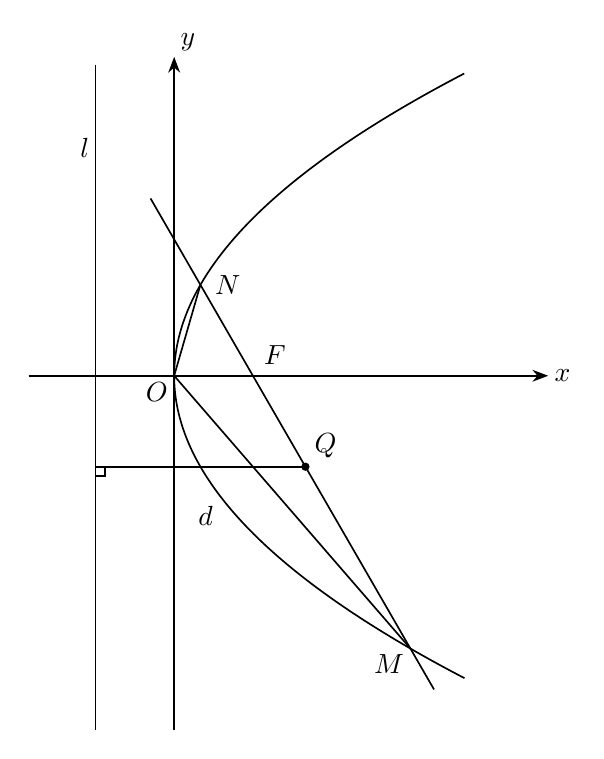
\begin{tikzpicture}[x=1cm,y=1cm,line width=.6pt,>=Stealth,font=\normalsize]
\coordinate (O) at (0,0);
\coordinate (F) at (1,0);
\coordinate (M) at (3,-3.4641);
\coordinate (N) at (0.3333,1.1547);
\coordinate (Q) at (1.6667,-1.1547);
\coordinate (DL) at (-1,-1.1547);
\coordinate (DLa) at (-0.88,-1.1547);
\coordinate (DLb) at (-0.88,-1.2747);
\coordinate (DLc) at (-1,-1.2747);
\coordinate (Ltop) at (-1,3.95);
\coordinate (Lbot) at (-1,-4.5);
\coordinate (Mtop) at (-0.3,2.2517);
\coordinate (Mbot) at (3.3,-3.9837);
\draw[domain=-3.84:3.84,samples=161] plot ({\x*\x/4},{\x});
\draw (Ltop)--(Lbot);
\draw (Mtop)--(Mbot);
\draw (O)--(M);
\draw (O)--(N);
\draw (Q)--(DL);
\draw (DL)--(DLa)--(DLb)--(DLc);
\fill (Q) circle (1.5pt);
\draw[->] (-1.85,0)--(4.75,0) node[right,inner sep=2pt] {$x$};
\draw[->] (0,-4.5)--(0,4.05) node[above right,inner sep=2pt] {$y$};
\node[anchor=north east,inner sep=0pt,xshift=-2pt,yshift=-2pt] at (O) {$O$};
\node[above right,inner sep=2pt] at (1.06,0.06) {$F$};
\node[anchor=north east,inner sep=0pt,xshift=-2pt,yshift=-2pt] at (M) {$M$};
\node[anchor=west,inner sep=0pt,xshift=5pt] at (N) {$N$};
\node[anchor=south west,inner sep=0pt,xshift=3pt,yshift=3pt] at (Q) {$Q$};
\node[left,inner sep=2pt] at (-1,2.9) {$l$};
\node[inner sep=2pt] at (0.4,-1.78) {$d$};
\end{tikzpicture}
